\documentclass[a4paper,11pt]{article}
\usepackage[style=mla,style=authoryear,backend=biber]{biblatex}
\renewcommand*{\nameyeardelim}{\addcomma\space}  % add comma between author and year
\usepackage{soul}
\usepackage{hyperref}
\usepackage[colorinlistoftodos]{todonotes}
\usepackage{calc}  % importent in order to import inkspace images
\usepackage[labelfont=bf]{caption}  % set caption label to bold
\usepackage{enumitem}  % to interrupt enumerations and resume
\usepackage{amsmath}
\usepackage{tabularx}  % alternative tabular package for the surveys
\newcolumntype{Y}{>{\centering\arraybackslash}X}  % for centered columns
\usepackage[toc,page]{appendix}

\addbibresource{bibliography.bib}

\graphicspath{ {images/}{graphics/}{plots/} }

\newcommand{\definition}[1]{\emph{#1}}
\newcommand{\noriinline}[1]{\todo[author=Nori,inline,color=green]{#1}}
\newcommand{\nori}[1]{\todo[author=Nori,color=green]{#1}}
\newcommand{\myunderline}{\rule{2in}{.5pt}}

\title{Audio-Only Augmented Reality System for\\Social Interaction}
\author{Tom Gurion}

\begin{document}
\maketitle

% \listoftodos
\tableofcontents

\section{Introduction}

Over the past sixty years the development of new technologies has fundamentally transformed music creation and consumption (\cite{hargreaves99}).
One result of these changes is the emergence of interactive music systems (IMS), which facilitate new ways of music creation by blurring the traditional distinction between instrument design, composition and performance (\cite{drummond09}).
In recent years there have been many attempts to provide IMS not only to professional musicians, but also directly to the average user (\cite{stimulant13}).

This research, in which I propose an audio-only augmented reality system for social interaction, aligns with this trend by exploring new possibilities for interactive music consumption, by a group of users, jointly.

The system is mainly motivated by silent disco, flash mobs and augmented reality, and aims to create an interactive space, in which users can move, interact, and affect thereby the music they and their companions hear in their headphones.
Throughout the research the system is presented by a silent disco use case.
Nevertheless, the system in characterized by an open architecture to allow different use cases and further exploration of the system's interactive behavior.

I have assessed the social effects of the system usage in two experiments, in the context of silent disco party, hypothesizing that it enhance social interaction between its users.
The results of the first experiment shows that indeed, the system facilitates higher social interaction between the users of the system.
Furthermore, the second experiment fine-tune the insights of the first experiment by presenting complex set of movement and gathering patterns.
These results are integrated to describe a model for the enhanced social interaction, thereby displaying the potential of using audio-only augmented reality in future interactive experiences.

\section{Literature review}

The current work is based on interdisciplinary research in several different domains.
The following sections will review those domains with emphasis on the projects, technologies, and research that serve as the ground for both the development and evaluation of my system.

In sections \ref{literature:ims} and \ref{literature:non_pro_ims} I will present the origins of IMS and recent trends relevant to my study.
Sections \ref{literature:social_tech} and \ref{literature:ar} present the motivation for the system development.
Some specific technological background for the system development, dealing with indoor positioning capabilities of mobile devices, is presented in section \ref{literature:ips}.
Finally, section \ref{literature:social_effects} shortly reviews the social effects of music and suggests a motivation for the evaluation of my system.

\subsection{The origins of interactive music systems} \label{literature:ims}

According to the Oxford Dictionary, to ``interact'' is to ``act in such a way as to have an effect on each other''.
In the field of IMS, actions and effects may be achieved by using a broad spectrum of novel techniques, ranging from interactive sound installations to collaborations with robotic performers (\cite{drummond09}).

Traditionally, IMS merges developments in several different threads to facilitate new ways of music creation.
Music-oriented programming languages as the MUSIC-N series and Max/MSP (\cite{mathews69}; \cite[p. 16]{winkler01}), standardization of technologies like MIDI (\cite{web:quinn}), the role of the personal computer in music production (\cite{leider:04}), and the recent emergence of the ``makers culture'' (\cite{kuznetsov2010rise}) are just a small sample of these threads.
Hence, considering the broad nature of the field, the current section will only briefly describe some of its historical highlights and doesn't meant to serve as an exhaustive overview.

Since early exploration in the field of IMS in the nineteen-sixties, different researchers and composers created systems that were designed to interact with performer in a live situation.
Perhaps the first example of this kind of interactive system is Gordon Mumma's Hornpipe, a specially designed electronic system that alters the audio input from the performer, creating an interactive loop between the player and the sound emitted by the electronics circuit (\cite[p. 12]{winkler01}).

During the nineteen-seventies, musicians and researchers started to use newly developed programming languages that was designed specifically for musical applications, such as GROOVE or the MUSIC-N series (\cite{mathews70}; \cite{mathews69}).
As pioneering technologies for digital sound synthesis, these programming languages gained wide acceptance in the music research community, serving as the roots for the new genre and field of research of computer music.

Charles Dodge's ``Earth's Magnetic Fields'' is one of the earliest computer music compositions, and thereby may serve as a good example to the new and unique possibilities it offers.
In this piece, magnetic field readings were collected over the course of a year.
Later, Dodge mapped the readings to a four octave span, applying interpolation between readings that manipulates the tempo and dynamics of the music (\cite{scriptsgrooves14}).
This attitude, in which the composer describes a set of rules and apply them on input data to generate musical materials automatically was impossible before, where the main technique to compose electronic music was by cutting and pasting magnetic tapes manually.

In 1983, a group of musical instruments manufacturers agreed on a universal standard for digitally sending and receiving musical information, establishing the MIDI protocol (\cite{web:quinn}).
This standardization, combined with the emergence of personal computers, facilitated the creation of modern programing languages for musical applications.
As opposed to early programming languages as GROOVE or the MUSIC-N series, most of the personal-computer-based languages still exist today and have kept progressing.
A prominent example is Max/MSP, which was first developed by Miller Puckette in 1986 (\cite[p. 16]{winkler01})\footnote{Max 6, the recent version of Max/MSP: \href{http://cycling74.com/products/max/}{cycling74.com/products/max/}.}.
Moreover, new music-oriented programing languages continue to be developed today, presenting features like ``on-the-fly'' programming\footnote{ChucK: \href{http://chuck.cs.princeton.edu/}{chuck.cs.princeton.edu/}.}, web capabilities\footnote{The Web audio API: \href{http://www.w3.org/TR/webaudio/}{www.w3.org/TR/webaudio/}.} or modular, multi-touch environment for live performance\footnote{Usine Hollyhock: \href{http://www.sensomusic.org/usine/}{www.sensomusic.org/usine/}.}.

Similar technological shifts also facilitated the usage of personal computers as a central component in the modern recording studio, thereby establishing its role as a common alternative to analog recording equipment (\cite{leider:04}).
With the arrival of VST as the common standard for digital signal processing plug-ins, computers became an even more essential tool for music production.
These developments were concurrent to the emergence of live performance-oriented software as Ableton Live\footnote{Ableton Live: \href{http://www.ableton.com/en/live/}{www.ableton.com/live/}.} and software based DJ setups at the late nineteen-nineties.

Another key event in the history of IMS is the appearance of the Arduino platform in 2006.
Arduino is an easy-to-use hardware and software package intended for interactive objects or environments creation\footnote{Arduino: \href{http://arduino.cc/}{arduino.cc/}.}.
By translating physical properties into sound, the Arduino platform opened the door for musicians to use more than just audio and MIDI to communicate with music creation software in interactive environments.

More generally, one can regard Arduino as an important part of the new ``makers'' movements, a technology-based extension of the ``do it yourself'' culture.
By creating what used to be purchased, and sometimes open-sourced it (sharing this knowledge back with the community), the makers have become a major driving force in the development of IMS (\cite{web:kirn12}).

Today, the makers movement can be seen as an unofficial host for several IMS projects by independent ``makers'', that present their works in different maker fairs around the world.
The large amount of dedicated web pages for musical projects in several websites that relate directly to the field can show how bound is the integration of musician with the makers community\footnote{Examples: \href{http://blog.arduino.cc/category/music/}{blog.arduino.cc/category/music/}; \href{http://makerfaire.com/category/music/}{makerfaire.com/category/music/}}.

\subsection{Interactive music systems for non-professional musicians} \label{literature:non_pro_ims}

These days, IMS meets the non-professional musician in various scenarios, including interactive video clips, mobile and album applications, interactive sound installations, and social DJing.
While these examples are typical, they are only a small portion of the novel ways in which non-professionals can now participate in interactive music creation and consumption of audiovisual content as well as musically enhanced social interactions.

% interactive video clips: Interlude, Chris Milk and Aaron Koblin
Interactive video clips share some of the roles traditionally kept for the director with the viewers.
As a relatively new phenomena, video clips like these have become increasingly prominent within popular culture.
A notable example are the works by Chris Milk and Aaron Koblin, in which the video clip runs on a dedicated webpage and responds to the users by tracking their mouse, keyboard strokes, or other inputs\footnote{Milk and Koblin's projects: \href{http://www.thewildernessdowntown.com/}{www.thewildernessdowntown.com/}; \href{http://www.ro.me/}{www.ro.me/}.}.
In Milk's project ``ROME - 3 dreams of black'', the user is presented with three dimension world, in which the video clip is occurring.
During the clip the user can choose a direction to stare at using the mouse, which also affects the visual image around the pointed area.
At the end, he / she is invited to create new three dimensional objects, using an editor in the browser, that will be added to the virtual world of the clip for future visitors.

A similar approach can also be found in interactive video clips created by the startup Interlude\footnote{Interlude: \href{http://interlude.fm/}{interlude.fm/}.}, Beck's recent project ``Hello again''\footnote{Beck's ``Hello again'': \href{http://www.hello-again.com/beck360/}{www.hello-again.com/beck360/}.} and more.
In contrast to ``ROME'', where the interaction with the video clip manipulate the visual output only, in the other projects mentioned above the manipulation is done on both the auditory and the visual domain.

% mobile applications: Smule and RjDj
Mobile phones, which were merely a communication tool until recently, are gaining more computational capability and comprehensive features each year.
These improvements change the way users interact with mobile devices and continuously contribute to the development of new IMS for non-professional musicians.
It is unsurprising though that the number of musical mobile applications that integrate interactive components are rising constantly.
For example, AutoRap turns speech into rap by slicing the syllables and mapping them according to different beat styles\footnote{Smule's AutoRap: \href{https://play.google.com/store/apps/details?id=com.smule.autorap}{https://play.google.com/store/apps/details?id=com.smule.autorap}.}.
Other examples are applications by Brian Eno and Peter Chilvers, which enable users to compose music using only visual elements on the device's screen\footnote{Generative music: \href{http://www.generativemusic.com/}{www.generativemusic.com/}.}.
Finally, RjDj uses the phones' sensors to create ambient sonification based on the users' interactions with their daily environment (\cite{web:rjdj})\label{rjdj}.

% album applications
Album applications are another new trend in which artists are releasing their music as interactive applications for mobile devices.
A notable example of this trend is the Icelandic musician Bj\"{o}rk's latest album, ``Biophilia'', which accompanies each of its 10 songs with a separated interactive experience (\cite{stimulant13}).
In Biophilia, the users are encouraged to interact with the musical materials visually to alter the compositional blocks (e.g. phrases and instruments) at wish.
In additional to this interactive mode, named ``play'' mode in the application jargon, there are other interesting modes in this album application that the user can choose from.
Score mode, for example, resemble some kind of karaoke, and animation mode, presents an animated video-clip of the song.

% interactive sound installations: objects with sound, project ADA
Sound installations are specific type of installations located in the three-dimensional space that communicate with their audience through sound.
In some interactive sound installations the main interaction is between the viewer and the installation itself (\cite{web:visnjic}; \cite{web:cardiff01}) whereas in others, the main objective is to facilitate social interaction between participants (\cite{eng03}; \cite{web:kirn12}; \cite{web:murray-browne13}).

% social DJing: DistributedDJ, the BLOB and playmysong
A number of recent projects suggest the framework of distributing the role of a DJ between participants so they can choose the music by themselves, thereby generating a playlist dynamically according to their musical tastes (\cite{web:shaw}), or distributing the DJ controllers between several participants, allowing each to control a different aspect of the music (\cite{web:shapira}).
Most of these project are implemented as mobile or web applications, and some of them even integrate social elements\footnote{Playmysong: \href{http://www.playmysong.com/}{www.playmysong.com/}; The BLOB \href{http://vimeo.com/7338120}{vimeo.com/7338120}.}.

\subsection{Technology dependent social networking} \label{literature:social_tech}

Silent disco and flash mobs, the conceptual roots of this project, are examples of modern types of social behavior that rely on the fast growth of social media and newly available technologies.
My proposal operates within the context of a silent disco party, and is inspired by flash mobs in its usage of new technologies to facilitate creative and artistic social interactions.

Silent disco is the phenomenon of partying where the music is heard through headphones instead of loudspeakers.
This new phenomena changes the possibilities of an ordinary party.
One example is to have two DJs spin completely different sets side by side at the same party, allowing each participant, who has two-channel wireless headphones, to decide which DJ to listen to\footnote{Headphone Disco: \href{http://headphonedisco.com/show.php}{headphonedisco.com/show.php}.}.
Another option is to have no DJ at all, letting each participant to choose what music to hear individually, through his or her mobile device and headphones.

Flash mobs are the public gathering of people organized through social media to jointly perform a short act.
The unique aspects of this relatively new phenomena have led researchers to suggest that the emergence of flash mobs is a significant event in the history of mobile communication (\cite{nicholson05}) and that it inherently reflects an artistic intent (\cite{brejzek10}).

\subsection{Augmented reality} \label{literature:ar}

According to Azuma ``augmented reality (AR) enhances a user's perception of and interaction with the real world''.
This concept usually relates to the visual modality: ``AR systems integrate 3-D virtual objects into a 3-D real environment in real time'' (\cite{azuma97}).

Today's augmented reality systems include wearable devices that can superimpose a computer-generated image on the users' view of the real world (e.g\ Google glass\footnote{Google glass: \href{http://www.google.com/glass/start/}{www.google.com/glass/start/}.} and Meta\footnote{Meta: \href{https://www.spaceglasses.com/}{www.spaceglasses.com/}.}) and applications for mobile devices for several purposes, ranging from driving aids (iOnRoad\footnote{iOnRoad: \href{http://www.ionroad.com/}{www.ionroad.com/}.}) to marketing (\cite{ikea}).

My work extends the definition of an AR system from the visual to the auditory modality, by sharing a similar motivation, which will apply differently.
In this study I refer to AR as a way to enhance the experience of the user using external elements that integrate into his / her physical environment using technological aids.
Using the above definition, and applied to this study, the ``enhancers'' are the musical materials the users hear through their headphones whereas the ``augmented experience'' refers to the enhanced social interactions.
More generally, this attitude toward AR may open the door for a more comprehensive experience of virtual environments.

\subsection{Indoor positioning systems} \label{literature:ips}

The system I propose requires the ability to locate the positioning of the users within an indoor environment.
As we will shortly see, this is a non-trivial requirement.

Today, the usage of outdoor positioning systems is unquestioned and achieved mainly by the General Positioning System (GPS) which is available in any modern mobile device.
On the other hand, indoor positioning systems (IPS) have not yet been standardized, and therefore are still unavailable to the average user (\cite{web:turetsky}).

Recent research states that WiFi is a favored technology among IPS for mobile devices.
WiFi-based systems can also enhance accuracy by applying inertial navigation using a device's additional sensors, such as its accelerometer, gyroscope, compass etc.\ (\cite{web:harrop}).
Note however that those solutions depend on the deployment of WiFi infrastructure in every indoor environment where positioning information in desired.

A relatively new technology in the world of IPS is the Bluetooth low energy (LE)\footnote{Bluetooth LE: \href{http://www.bluetooth.com/Pages/low-energy-tech-info.aspx}{www.bluetooth.com/Pages/low-energy-tech-info.aspx}}.
Using this technology, supported devices can roughly approximate the distance of nearby mobile tokens within a radius of 10 meters or so.
Bluetooth LE has already gained success with the adaption of the technology by Apple with their iBeacon IPS (\cite{web:danova});
Estimote\footnote{Estimote: \href{http://estimote.com/}{estimote.com/}.}, one of the biggest iBeacon manufacturers, has recently reported that more then 10,000 developers are using their products (\cite{web:thompson});
StickNFind use the technology similarly\footnote{StickNFind: \href{https://www.sticknfind.com}{www.sticknfind.com}.};
Android has introduced built-in support for Bluetooth LE\footnote{Android Bluetooth LE: \href{http://developer.android.com/guide/topics/connectivity/bluetooth-le.html}{developer.android.com/guide/topics/connectivity/bluetooth-le.html}.} and there is even an Arduino shield (standard board extension) for it\footnote{Arduino Bluetooth LE shield: \href{http://redbearlab.com/bleshield/}{redbearlab.com/bleshield/}.}.

\subsection{Social effects of music} \label{literature:social_effects}

% Explain what does it means social effect of music.
Music is known for being an important channel of communication.
It is therefore unsurprising that the function of music in everyday life have been extensively studied.
Questions about music functionality can arouse in various disciplines, ranging from psychological to anthropological studies.
The following is a narrowed down review of the most essential parts of this field to my study.
Namely, I will try to concentrate on studies that describe music as a social function, exploring the ways music can reshape social structure or affect ones sense of belonging to a group.

% Self-identity (Hargreaves and North; Cook) and personality dimensions (Rentfrow and Gosling). Demonstrate.
Hargreaves and North suggest that the psychological functions of music may be best understood as social effects on the individual (\cite*{hargreaves99}).
They describe a framework in which those effects are classified by means of self-identity (e.g. teenagers that join musical subcultures as a means of defining themselves), inter-personal relationships (e.g. client-therapist relationship in music therapy context) and mood (e.g. influences on costumers behavior in shops and stores).
Nicholas Cook use the youth generation of the ninety-sixties as an example of a social phenomena motivated by a prominent musical cause (\cite*[p. 5]{cook00}).
Using Hargreaves and North methodology one can say that music is a significant component in the self-identity of the members of the youth generation.
A summary of this attitude can be put by Cook's words: ``People think through music, decide who they are through it, express themselves through it'' (\cite*{cook00}).

Indeed, experimental studies have supported the assumption that music affects self-identity and inter-personal relationships by showing a high correlation between musical preferences and a wide array of personality dimensions (e.g.\ conscientiousness and openness) as well as self-views (e.g.\ political orientation) (\cite{rentfrow03}).

% Music's synchronization characteristics emphasize group level effects (Brown).
From another point of view, researchers suggest that music originally evolved as a device to support group functions (\cite{Brown2000}).
This hypothesis is supported by a wide range of universal characteristics of music, such as isometric rhythm and discrete pitches, all emphasizing coordination and synchronization in the group level.
According to Brown ``music acts as an emotive enhancer of cultural objects other than itself'' (p. 236).
Meaning that, in a given society, musical materials are always associated with external cultural ideas, that can be perceived by the groups' members.
Prominent examples are rituals, demonstrating that the music functions on the group level (as opposed to on the individual level) by enhancing some non-musical concept ---  religion, for example.

% Furthermore, in-group vs. out-group effects (Brown; Hagen)
Furthermore, Brown claims that music's group functionality can be described with regard to both within-group cooperation, promoting group identity and cohesion, as well as between-group competitiveness.
Brown's research operate in the field of evolutionary studies, whereby the fitness benefits of a trait are always of high interest.
With that idea in mind, he argues that ``Music's fitness advantages come about from its ability to promote group-wide cooperation, coordination, cohesion and catharsis, and this operate to increase both group welfare and group warfare'' (p. 257).

Hagen and Bryant extend Browns' ideas by suggesting that music and dance originally evolved as a signaling system for the existence, as well as the quality, of a coalition between individuals, noting that humans are the only primate to create cooperative alliances between groups in the absence of consanguineous ties (\cite*{Hagen2003}).

% joint action
% use Kirschner & Tomasello 2010 and Knoblich et al. 2011
Recent studies show that joint music making and dancing can indeed increase group cohesion, pro-social commitment among the individuals of the group, and the intent to share the same collective goals (\cite{Kirschner2010}; \cite{Knoblich2011}).

% Linking to my study
In this research I will evaluate the social effects of a system for interactive music consumption, by assuming priors and hypothesizing effects based on the studies above.
Throughout this text I will use the notions ``in-group cohesion'' and ``openness to out-group interactions'' extensively, resembling to Brown's description of within-group cooperation and the negation of between-group competitiveness.
Whereas most of the studies above (Brown's included) demonstrate how music increase in-group cohesion and \emph{decrease} openness to out-group interactions, my proposed system aims to promote interaction outside the native social groups.

\section{Research targets}

In this research I will focus mainly on two distinct but complementary targets.

\begin{enumerate}[resume]
    \item I will propose and implement an audio-only augmented reality system for social interaction.
          The system will be designed to be used by a group of users, together, in the same space and time.
          It will consist of mobile application --- which will be eventually installed on each of the users' mobile devices --- and several mobile tokens, spread in space.
          The users will be able to stroll with their mobile devices, interact with the mobile tokens and therefore affect the sound they and their companions hear in the headphones.
          The interactive component of the system will facilitate social interaction between users, based on joint interactions with the mobile tokens.

    \item I will evaluate the social effects of the system usage within the context of a silent disco party, focusing thereby on the main research question: \emph{does the system enhance social interaction between participants in an interactive silent disco party?}

          In the experiments below this research question will break down into more specific and testable measures, assessing whether participating in a party using the system (a) strengthens the social relationships between participants even beyond the scope of the experiment and (b) alter in-group cohesion and ones openness to out-group social interactions.
          Motivation for these will be clarified by the results of experiment 1.
\end{enumerate}

In addition to the two main targets presented above, the following secondary targets will be assessed as well:

\begin{enumerate}[resume]
    \item I will aim to develop the system with open architecture in mind in order to enable other musicians and researchers to use my system for their own purposes.
          The openness of the system architecture will be expressed throughout several different aspects, from platform and hardware decisions such as Android and Bluetooth, which are both widely common, to the design of the application itself, which will separate concerns between musical materials, audio engine and the logic that tide them together.
    \item I will try to show correlation between different types of measurements analyzed during the evaluation of my system.
          More explicitly, I will compare the results gathered using surveys to those of objective measurements as Bluetooth readings and video tracking.
          Correlated results may both enhance the credibility of my findings significantly and show that social behavior can be assessed by subjective and the objective measurements alike.
\end{enumerate}

\section{System development}

In this section I explain the rationale for the choices of system development in the context of the above research targets, and describe the details of system implementation.

\subsection{Mobile and Android}

Today's mobile phone has transformed from being a communication tool into a key `social object' within everyday life, and as such it has significant importance in shaping contemporary society (\cite{srivastava05}).
As the applications of this research are targeted at the general audience, the entire research is implemented for mobile.

The system was developed for the Android operating system\footnote{Android OS: \href{http://www.android.com/}{www.android.com/}.}.
Choosing Android as the platform for my research has two main advantages:
\begin{itemize}
	\item The Android system is a growing mobile system which dominates most of the market share today (\cite{web:idc}).
	\item By developing an application for Android, I could access underlying Bluetooth properties such as received signal strength indicator (RSSI), which is essential for my implementation of the system as laid out in the following section.
\end{itemize}

\subsection{Indoor positioning system}\label{methods:ips}

Although there are available techniques to implement IPS, I decided to develop a novel method from the following reasons:

\begin{itemize}
	\item Most of the techniques available nowadays require infrastructure.
	As a system influenced by flash mobs, I wanted users to be able to use it anywhere without the effort involved in infrastructure deployment.
	\item Tracking the positioning of the participants is only required within the context of their relative position to some other mobile tokens in the system, therefore we do not need to track the absolute position of each participant in space (the ``world'' coordinate of their position).
	\item As opposed to a system where high accuracy is required, the current research needed only limited accuracy.
	Being able to estimate if a participant is relatively close to or far from another mobile token was generally sufficient.
        \item Although Bluetooth LE based solutions satisfy the all of the above requirements, only the most recent mobile devices support them. In fact, the technology was not yet available during the initial phases of the system development, whereas my Bluetooth based solution, as described below, behaves similarly but still supports a wider range of mobile devices.
\end{itemize}

The indoor positioning system I developed --- the Bluetooth Based Relative Indoor Positioning (BBRIP) system --- consists of a number of Bluetooth beacons and an Android application.
It is built around distributed architecture and therefore runs separately as an Android application, on each one of the participants' phones.
The application repeatedly searches for nearby Bluetooth beacons.
The RSSI value is used as an estimation of the distance between the user and the beacon.

\subsection{libpd}\label{methods:libpd}

Advanced audio processing is beyond the capabilities of the Android application programming interface and therefore, in order to apply sophisticated manipulations on the audio in real time, a more powerful audio engine was required.
In a personal computer environment the programming language Pure Data (Pd), originally written by Miller Puckette in the nineteen-nineties, is a leading open-source software for computer music\footnote{Pd: \href{http://puredata.info/}{puredata.info/}.}.
In this project I decided to use ``libpd'', a thin layer on top of Pd that turns it into an embeddable audio library, as an audio engine (\cite[p. v]{brinkmann12}).

\subsection{System description}\label{systemdescription}

\begin{figure}[!htb]
	\centering
	\def\svgwidth{0.9\textwidth}
	\input{graphics/system_architecture.pdf_tex}
	\caption{System architecture}\label{fig:sys:architecture}
\end{figure}

Figure \ref{fig:sys:architecture} shows a schematic diagram of the system, which consists of an Android application and specially designed Bluetooth beacons ($BB1 - BB4$).
The BBRIP system is used to estimate the distance between the user and nearby Bluetooth beacon.
This estimation is then sent to a Pd patch through libpd, which plays an audio loop corresponding to the nearby beacon by one of the sound zone players $SZP1$ -- $SZP4$.
Every audio loop is identified by a distinct musical style which can be rhythmically and harmonically synchronized with other loops in almost endless combinations.

\begin{figure}[!htb]
	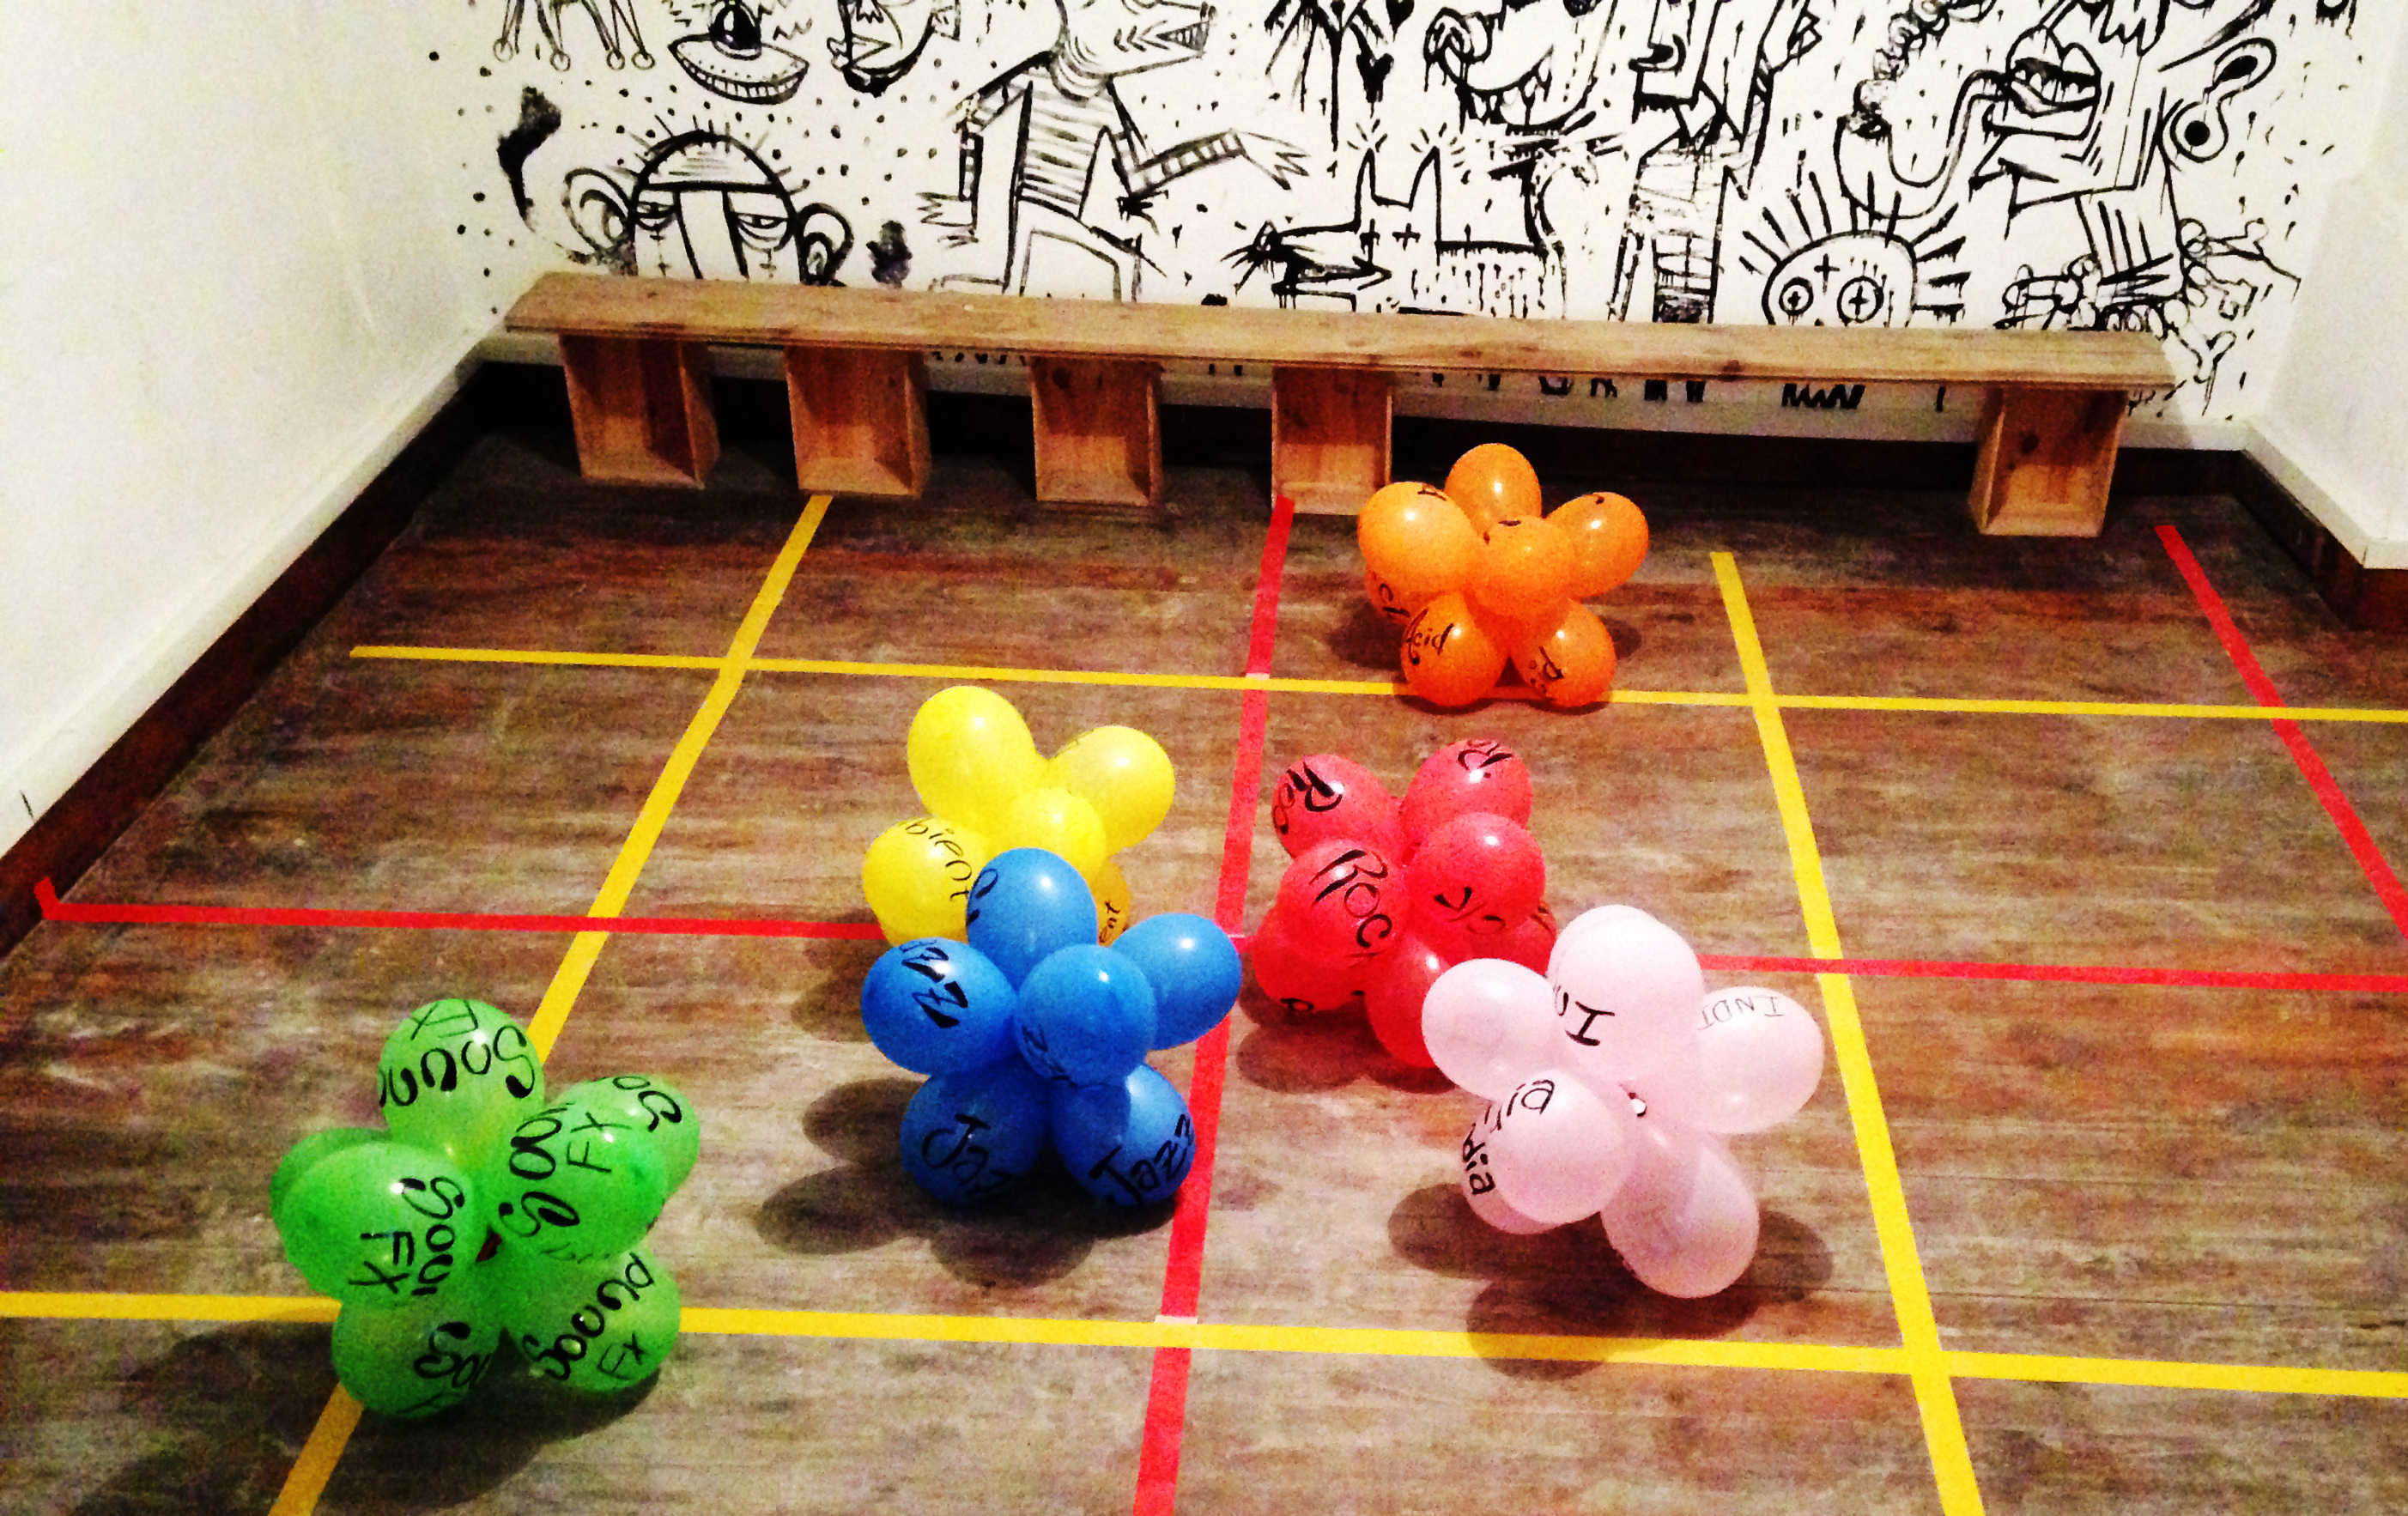
\includegraphics[width=\linewidth]{balloons}
        \caption{Balloon bundles on the dance floor (experiment 1)}\label{fig:balloons}
\end{figure}

Figure \ref{fig:balloons} shows the system's elements on the dance floor.
It consists of few balloon bundles, each marked with the name of a specific musical style (e.g.\ rock, jazz, Indian music).
A corresponding Bluetooth beacon is installed inside each of these bundles.
After downloading and installing the Android application, strolling between the balloon bundles affects the music in one's headphones according to the relative distance from the bundles, creating a virtual ``sound zone'' around each of them.
In addition, the distance from the center of each sound zone may affect the music in several different ways; for example, by controlling the volume, filter, and granularity of the sound zone.
Lastly, participants can move the balloon bundles freely, thereby dynamically changing the structure of the music in the virtual space and making it socially interactive.

Figure \ref{fig:sys:participant_view} shows an overhead view of a possible scenario of participants using the system in a party.

\begin{figure}[!htb]
	\centering
	\def\svgwidth{0.9\textwidth}
	\input{graphics/system_participant_view.pdf_tex}
	\caption{The figure shows schematically two participants, $A$ and $B$, dancing around three Bluetooth beacons, corresponding to the rock, jazz, and Indian music sound zones. Participant $A$ hears rock music and participant $B$ hears a mixture between the jazz and the Indian music sound zones, which are rhythmically and harmonically synchronized with each other. A video demonstration of a similar scenario can be found at \href{http://youtu.be/2kJoeD2iWBA}{youtu.be/2kJoeD2iWBA}.}\label{fig:sys:participant_view}
\end{figure}

\subsection{The BBRIP system}

The implementation of the system can be described by two different processes: the development of the BBRIP system (described in this section) and the Android application that wraps it and is responsible for the audio processing (see section \ref{sceneplayer_plus}).

The BBRIP system is my intent to develop an indoor positioning system that satisfies the relatively simple requirements of the research as presented in section \ref{methods:ips}.

My implementation of the system is based on a specific element in the Bluetooth protocol -- the Received Signal Strength Indicator (RSSI) ({\cite{bray12}).
Each Bluetooth enabled device calculate RSSI values during Bluetooth discovery, when it finds a new device and before establishing connection.

\begin{figure}[!htb]
	\centering
	\def\svgwidth{\columnwidth}
  	\input{graphics/bbrip.pdf_tex}
	\caption{The BBRIP system states and flow design}\label{fig:bbrip}
\end{figure}

As shown in figure \ref{fig:bbrip}, the BBRIP system continuously searches for Bluetooth devices.
When a new device is found, the RSSI value is extracted and sent forward for processing.
From the first discovery in the Bluetooth discovery cycle, the system keeps checking if the time since the last discovery exceeds a pre-defined timeout.
If so, it terminates the discovery.
This termination is important, because naturally a device can only be discovered once in each Bluetooth discovery cycle, and long periods of time without new discoveries indicates that all of the nearby devices have already been found.
Lastly, when the system sees that there is no Bluetooth discovery running (because of termination or simply the end of the discovery cycle), it starts a new one immediately.

Although the RSSI values extracted by the BBRIP system are not very precise as a distance estimation, I have found them sufficient in order to classify the distance between participants and beacons into useful ranges.
In other words, RSSI values gives great indication if a participant stands close to specific beacon (around 1 meter), in an intermediate range (2 to 3 meters), or in a greater distance.

\subsection{ScenePlayer Plus}\label{sceneplayer_plus}

The development of the Android application moved through different development stages.

In the first phase of the development the audio files that was used for playback were built into the application code-base, making the application tightly bound to a specific set of sounds and interaction opportunities.
In this early stage the application didn't use ``libpd'' at all (see section \ref{methods:libpd}).
Therefore, the only effect of approaching or leaving a beacon was a change in volume.
In addition, the limited sophistication of the built-in audio library made fading in and out from the sound zones very inflexible.

After finding the weakness of the built-in audio library of the Android application programming interface, I decided to implement the system using ``libpd''.
The shift toward ``libpd'' open the possibility to use more advance audio manipulations, instead of only volume changes, including, for example, filtering and granular synthesis of the audio sources.
Although the framework change presented an improvement, there was still very tight coupling between the system development in the Android environment and the audio processing development in Pd.
This tight coupling is expressed by the fact that the audio sources was still embedded in the application code-base, as well as the Pd patch, meaning that other musicians and researchers was still unable to load different musical materials and different Pd patches to change the behavior of the system for their artistic nor academic desire.

Overall, this development phase was sufficient for answering the main research questions.
Nevertheless, I have started to search for a better, more open, architecture.
An architecture that maintains a loosely coupled connection between the Android application, the musical sources, and the Pd patch that drives the audio, and which will allow others to use the system easily.

The last phase in the system development was to implement the BBRIP system into the open source Android application ``ScenePlayer''\footnote{ScenePlayer: \href{http://play.google.com/store/apps/details?id=org.puredata.android.scenes}{play.google.com/store/apps/details?id=org.puredata.android.scenes}.}, an Android port for the RjDj application mentioned in section \ref{rjdj}, and release it again as ``ScenePlayer Plus''\footnote{ScenePlayer Plus: \href{https://github.com/Nagasaki45/ScenePlayer-Plus}{github.com/Nagasaki45/ScenePlayer-Plus}.}.
`Scenes' in ScenePlayer are bundles of audio files and one or more Pd patches that describe, programatically, how input from the mobile device sensors should affect the audible output (\cite[p. 29]{brinkmann12}).
This design allows musicians to create Pd patches that can be uploaded to the mobile device, along with extra audio materials, to create sophisticated interaction easily.
In ScenePlayer Plus, the BBRIP system is used to expose the received Bluetooth RSSI values to the Pd patch as another sensor of the mobile device (e.g.\ accelerometer, compass and touchscreen)\footnote{The scene that was used for the this research can be found at my site: \href{http://tomgurion.blogspot.com/2013/06/arparty-first-sceneplayer-plus.html}{tomgurion.blogspot.com/2013/06/arparty-first-sceneplayer-plus.html}.}.

\section{Experiment I}

In order to evaluate the social effects of the system's usage I decided to conduct controlled experiments.
For the sake of evaluating the system in its most natural designation, the context of the experiments was selected to be a silent disco party.
The experiments' main goal is to answer the research question: \emph{does the system enhance social interaction between participants in an interactive silent disco party?}

In addition, two additional hypotheses are that participating in a party using the system (a) strengthens the social relationships between participants even beyond the scope of the party and (b) alter in-group cohesion and ones openness to out-group social interactions.

Assessing the social interaction between participants was done using two main methods: by self-reported information that the participants entered in surveys before, during, and after each experiment, and with objective measurements such as participants positioning tracking and their interaction with system components.
Another target of this study is to evaluate the correlation between the results of these different methods.
Positive results in this aspect will greatly enhance the credibility of my findings and more generally, may confirm the implied hypothesis that social behavior can be assessed using the participants' self-reported information and objective measurements alike.

The following sections present the first experiment that has been conducted, presenting detailed explanation of the experimental design and its results.

\subsection{Methods}

\begin{figure}[!htb]
	\centering
	\def\svgwidth{0.95\columnwidth}
  	\input{graphics/pilot_design.pdf_tex}
	\caption{Pilot experiment design}\label{fig:pilot}
\end{figure}

Eighteen volunteers were invited to participate in an interactive silent disco party.
Each participant installed the Android application on his or her phone and filled pre/post party surveys that included questions regarding their musical background and preferences as well as system evaluation feedback.
The party consisted of four alternating interactive/control sessions of duration 5:40 minutes each (see figure \ref{fig:pilot}).
The participants were randomly assigned to two groups: $A$ and $B$, comprising the interactive and control sessions respectively\footnote{Group $A$ (interactive first) consisted of 8 participants (4 females and 4 males) with mean age of 36.7 (s.d=12.3); group $B$ (control first) consisted of 10 participants (3 females and 7 males) with mean age of 29.6 (s.d=10.2). Participants had a diverse musical background with 4.7 mean years of musical training (s.d=5.2).}.
They were informed that the experiment consists of interactive and control segments, however, they were not informed about the exact schedule and timing of the sessions or the group assignments.
Both groups started the experiment together, and on the same dancing floor.
In the interactive sessions, the application generated music as described in section \ref{systemdescription}, whereas in the control sessions the participants heard recorded non-interactive music created in advance using the musical material of the interactive system\footnote{The control session music composed by Noam Elron (\href{http://www.noamelron.com}{www.noamelron.com}).}.

Interaction with the system's components was assessed by counting the number of Bluetooth device discoveries made by each participant's phone during both the interactive and the control sessions.
In order to eliminate edge effects, I analyzed sensor data only from the two middle sessions of the experiment.

\subsection{Results}

\begin{figure}[!htb]
\minipage{0.49\textwidth}
	\def\svgwidth{0.95\columnwidth}
  	\input{graphics/changing_location_in_space.pdf_tex}
	\caption{Changing location in space}\label{fig:location}
\endminipage\hfill
\minipage{0.49\textwidth}
	\def\svgwidth{0.95\columnwidth}
	\input{graphics/dancing_with_known_people.pdf_tex}
	\caption{Dancing with known people}\label{fig:known}
\endminipage\hfill
\end{figure}

In the post-party survey, participants self-reported significantly higher levels of movement (paired t-test, $t(15)=3.9$, $p<0.01$) using the system, compared with their behavior at other parties as reported in the pre-party survey.
Figure \ref{fig:location} shows that there was a significant difference (unpaired t-test, $t(33)=6.2$, $p<0.01$) in the mean response to these questions (at a scale of 1-3).

In order to objectively assess if participants moved more in space, I measured the counting of Bluetooth discoveries made by the applications' BBRIP system.
The results show slightly higher counts (paired t-test, $t(16)=1.7$, $p=0.06$, n.s) during the interactive sessions of the party compared with the control sessions.
This suggests that the interactive components of the system facilitated greater participant movement in space, thereby offering more frequent opportunities for social interactions.
Indeed, in the post-party survey participants reported that they danced significantly less with people that they knew in advance, compared with their usual behavior (paired t-test, $t(14)=-2.5$, $p=0.01$).
Figure \ref{fig:known} shows that there was also a significant difference in the mean response to these questions in the pre/post surveys.
Overall, participants showed a slightly stronger tendency (paired t-test, $t(16)=1.46$ ,$p=0.08$, n.s) to participate in an interactive party in the post-party survey, compared with their answer to identical question in the pre-survey.

\subsubsection{Video analysis}\label{exp1:results:video}

\begin{figure}[!htb]
	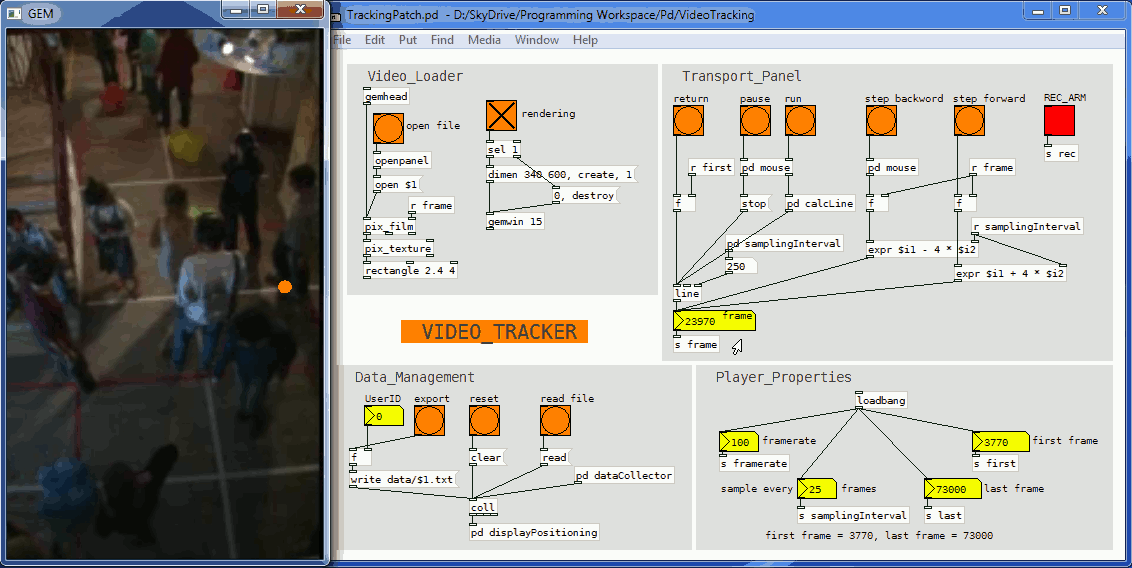
\includegraphics[width=\linewidth]{tracking}
        \caption{Pd patch for manual video tracking or participants on the dance floor}\label{fig:tracking}
\end{figure}

\begin{figure}[!htb]
    \centering
    \includegraphics[width=0.8\textwidth]{plots/pilot-familiarity_correlation_maps.pdf}
    \caption{Maps of social familiarity (on the left) and correlated movement on the dance floor (on the right)}\label{plot:pilot-familiarity_correlation_maps}
\end{figure}

The whole experiment was captured with video from above the dance floor.
Later, this video was used to track the positioning of the participants and to generate positioning tables ($x$ and $y$ coordinates on the dance floor per timestamp).

Figure \ref{fig:tracking} present the Pd patch I wrote to manually track the participants' movement on the dance floor.
Using this patch, I have tracked the positioning of each participant at a time with the computer mouse.
The location of the mouse pointer within the video window was recorded once for every 25 video frames (\textasciitilde{}1 per second)\footnote{In the second experiment positioning was captured twice per second.}.
Later, I used three points on the dance floor which have been measured for their real (although relative) coordinates in advance, to project the mouse tracking measurements from the video frame onto two dimensional coordinates on the dance floor.

Analyzing this data, I didn't find significant difference between the position and movement patterns in the interactive and control sessions.
However position was indicative to the social relations between participants.
I asked participants for their social relationships to other participants and compared the resulted map with a map of positioning correlation between every two participants, over the entire course of the experiment\footnote{This data was measured along the Y axis alone, which was much more indicative then the X axis due to the fact that the length of the dance floor (the Y axis) was 10 meters while the width of it was only 2.5 meters.}.
I defined the matrix similarity metric as the component-by-component squared distance and used bootstrapping resampling (\cite{good2006permutation}) to check how similar are those maps.
As expected, I found that the matrices are unusually similar (p \textless{} 0.001).

To conclude, the result above demonstrate how close social relationship between participants can also be found in video analysis data.
This encouraging results drove much of the methods to analyze the social behavior in experiment 2.

\subsection{Discussion}

The results already support the hypothesis that the system usage enhances the social interaction between participants.
They demonstrate the potential for audio-only augmented reality to significantly enrich the experience of music consumption and its attendant social interaction.
Furthermore, they also show that the research targets in question can be validated in a controlled experiment using both direct reports of subject and indirect objective measurements, and that video tracking analysis can be used to conclude social relationships.

However, the results does not shed a light on the following points:

\begin{itemize}
	\item It does not distinguish between participants that knew one another in advance.
	\item It does not show that the social effects of the system extends beyond the scope of the system usage.
\end{itemize}

A second experiment will therefor focus on clearing up these points.

First, in the following experiment I will assume that participants in a party are pre-partitioned into groups of friends.
This assumption is supported by the results of the video analysis, which shows that participants that are socially close tend to be together on the dance floor.
In addition, the same results also show a well defined social clusters.
Combining the above assumption and the ability to define social clusters based on social relationships between participants I will define \definition{in-group} and \definition{out-group} as group of members in a social cluster a participant belong to, and the rest of the participants respectively.
Thereby, in the following experiment a major effort will be made to gain better understanding of the behavior of those groups as a whole and the behavior of each participant as a member of a group.

Second, in the following experiment I will suggest a design in which the control group will not experience the interactive part of the system at all.
Thereby, the social behavior of the control group participants may be compared to the experiment group before and after the experiment to gain insights about the long term social effects of the system.

\section{Experiment II}

A second experiment was conducted based on insights gathers from experiment 1.
It aims to clarify some of the research targets that was not yet answered sufficiently and is meant to achieve fine-grained insights about the social effects of the system.

\subsection{Methods}\label{methods:evaluation}

\subsubsection{Participants}

An homogeneous class of twenty-three 11th grade pupils participated in the experiment.
The high-school was supportive and open the possibility to run the experiment with the pupils, using its facilities\footnote{An ethics certificate describing a highlighted procedure of the experiment was signed by a parent for each of the pupils who was under 18 age old.}.

\subsubsection{Measurements}

The research questions was fragmented into the following operational definitions and measurements\footnote{Complete version of each of the surveys can be found in the appendix.}:
\begin{enumerate}
	\item \label{measure:survey:familiarity} Participants reported their familiarity with other participants using a survey based on the experimental ordinal number.
	\item I have intended to use the above familiarity data to cluster the participants into social groups.
            Using this clustering and the participants positioning information (measured by video tracking as explained in section \ref{aparatus}) I was able to define the centroid of each cluster on the dance floor, disperse of participants within each cluster and the disperse between the clusters centroids themselves for each frame of the video.
            As you will shortly see in section \ref{results:social_structure}, I failed to find distinct social groups based on the familiarity surveys above.
        \item \label{measure:movement} Following positive results from experiment 1 movement assessment I have measured the average movement speed of the participants, hypothesizing that greater participants movement on the dance floor may offer more frequent opportunities to social interaction.
        \item \label{measure:clustering} For each frame of the video, I have dynamically clustered the participants into groups based on their positioning.
            Then, I have assigned scores to the clusters based on social and positional data in order to gain better understanding of the gathering patterns of the participants.
            Detailed explanation of the techniques used for clustering can be found in section \ref{results:clustering}.
	\item \label{measure:survey:social} Participants filled out a social interaction survey.
	The survey was used to asses interaction between participants by estimating social cohesiveness within in-group and openness to out-group interactions of each participant.
\end{enumerate}
In addition to measurements intended to assess the main research questions, the following operational definitions and measurements was used to assess interaction with and satisfaction from the system.
\begin{enumerate}[resume]
	\item \label{measure:system} I have measured and calculated the expected number of participants around a Bluetooth beacon to assess participants' interaction with the system's components, where more participants around a beacon indicating greater interaction.
	\item \label{measure:survey:usability} Participants filled out a system satisfaction survey, based on the System Usability Scale (\cite{brooke96}).
\end{enumerate}
Lastly, the following measurement was used in order to eliminate possible differences between research groups and to allow future research based on the retrieved data.
\begin{enumerate}[resume]
	\item \label{measure:survey:musical} Participants filled out a musical background survey, based on the Emmanuel College Music Background Questionnaire, basic version (\cite{web:zhao12}).
\end{enumerate}

\subsubsection{Apparatus}\label{aparatus}

Considerable number of the measurements described above require spatial participants positioning information.
In order to derive this kind of positioning data I have captured the experiment with a video camera from above the dance floor during the entire course of the experiment.
Extracting the positioning of the participants was done semi-manually, after the experiment, by tracking one participants at a time using the computer's mouse as explained in section \ref{exp1:results:video}.
The results was then processed using computational programming to conclude insights from the data.

The Bluetooth beacons positioning data required for measurement \ref{measure:system} was derived similarly, by manually tracking each of the system components in the video.

\subsubsection{Procedure}

Participants was randomly assigned to two groups, group $A$ and group $B$\@\footnote{Group $A$ consisted of 11 participants (5 females and 6 males) with mean age of 18.7 (s.d=5.41); group $B$ consisted of 12 participants (3 females and 7 males) with mean age of 17.2 (s.d=0.42). Participants had a diverse musical background with 4.17 mean years of musical training (s.d=2.53).}.
Each group participated in the experiment in different week, but on the same day of the week and same hour. Group $A$ participated first and two weeks later group $B$ was participated in the experiment.

\begin{figure}[!htb]
	\centering
	\def\svgwidth{0.9\textwidth}
  	\input{graphics/procedure.pdf_tex}
	\caption{Experiment design}\label{fig:experiment}
\end{figure}

First, participants filled a musical background survey (measurement \ref{measure:survey:musical}) and a participants familiarity survey (measurement \ref{measure:survey:familiarity}), followed by three \definition{experiment sessions}, followed by a system usability survey (measurement \ref{measure:survey:usability}).
After filling out the system usability survey the participants experienced another experiment session.
Before each experiment session and after the last one each participant filled the social interaction survey (measurement \ref{measure:survey:social}).

In each experiment session the participants listened to music in their headphones, using their Android device and pre-installed application, and interacted with other participants and system components in the `silent disco' party.
The type of an experiment session could by as following:

\begin{description}
	\item[Interactive:] In which the music generated by the Android application behaves as described in section \ref{systemdescription}.
	\item[Control:] In which the music generated by the Android application is semi-randomize sequence of the same musical materials that was used in the interactive system.
        The music in the control sessions was not affected by the positioning of the participant neither from the Bluetooth tokens in any way.
\end{description}

Participants of group $A$ heard the experiment sessions: Control $\rightarrow$ Control $\rightarrow$ Control $\rightarrow$ Interactive.
Whereas participants of group $B$ heard the experiment sessions: Control $\rightarrow$ Interactive $\rightarrow$ Control $\rightarrow$ Interactive, as shown in figure \ref{fig:experiment}

The procedure described above presents several advantages in assessing the research questions compared to experiment 1 design and variants of A / B designs.
First, the comparison between the effects of interactive and control sessions can be done as a between-group evaluation in relation to the second experiment session of each group.
Second, comparison between interactive and control sessions effects could also assessed as a withing-group evaluation between the first and the second, as well as the second and third sessions of group $A$, using group $B$ as a reference.
Lastly, effects on the social interaction beyond the scope of the interactive sessions can be assessed as a within-group evaluation between the first and the third sessions of group $A$, using group $B$ as a reference.

As one can see, all of the data required for analysis was already collected in the first three experiment sessions.
However, the last session was added to the experiment to prevent frustration and sense of discrimination between the groups.
Therefor, and despite the fact that the last session was not contributed to the collected data, it was very significant in preventing group $A$ participants from bias group $B$ results, as they all socially close\footnote{Group $A$ participants were asked not to discuss about the experiment with group $B$ participants.}.

\subsection{Results}

\subsubsection{System satisfaction surveys}

\begin{figure}[!htb]
    \centering
    \includegraphics[width=0.6\textwidth]{plots/usability-sus_scores.pdf}
    \caption{Mean system satisfaction scores for the control and interactive groups}\label{plot:usability-sus_scores}
\end{figure}

\begin{figure}[!htb]
    \centering
    \includegraphics[width=\textwidth]{plots/usability-per_question_statistics.pdf}
    \caption{System satisfaction questionnaire results. Bars indicates the mean response of single questions (questions are listed to the right).}\label{plot:usability-per_question_statistics}
\end{figure}

I used a system satisfaction survey at the end of the experimental session for each of the groups in order to evaluate the engagement of the participants with the system.
The survey was based on the standard system usability scale (SUS) survey (\cite{brooke96}) with minor modifications.
The SUS survey contain 10 question, 5 of them positive (a larger number indicates larger satisfaction) and 5 of them negative (a larger number indicates smaller satisfaction).
I used a score which combines positive and negative questions as suggested by Brook (\cite*{brooke96}).
Figure \ref{plot:usability-sus_scores} shows that the overall system satisfaction score is larger in the interactive group (interactive: 67.3 (3); control: 45.2 (6.9); unpaired t-test, t(21) = 2.81, p \textless{} 0.01).

This effect was not limited to a single question.
In fact, four of the ten questions showed significantly higher satisfaction response in the interactive group as indicated by a separated one-tailed t-test (p \textless{} 0.05). All questions but two showed some tendency (p \textless{} 0.1), and the remaining two questions (extended learning in question 10 and technician aid in question 4) are expected to be less relevant to this system.
These results are summarized in figure \ref{plot:usability-per_question_statistics}.
Overall, the results consistently show that subjects that used the interactive component of the system were more satisfied than the control group that had similar physical conditions.

\subsubsection{Social interaction surveys}

\begin{figure}[!htb]
    \centering
    \includegraphics[width=\textwidth]{plots/interaction_surveys-question_2.pdf}
    \caption{Mean participants response to social interaction statements; statement 1: ``In the last experiment session I interacted with close friends only''; statement 2: ``In the last experiment session I interacted with participants with them I have no social connection''}\label{plot:interaction_surveys-question_2}
\end{figure}

One of my main hypotheses was that the system will increase social interaction outside the native groups.
Namely, subjects that usually interact less with each other will tend to interact more.
To assess this hypothesis I have used social interaction survey between each of the experiment sessions.

Surprisingly, the results of this survey showed a different trend.
The left side of figure \ref{plot:interaction_surveys-question_2} shows the mean response (on a scale of 1 to 5) to the statement ``In the last experiment session I interacted with close friends only''.
There was no significant main effects and group by session interactions as indicated by 2-way repeated measure ANOVA (group: F(1, 21)=0.094 p=0.762; session: F(2, 42)=0.835 p=0.441; interaction: F(2, 42)=0.548 p=0.582).

Similar results were obtained for the second question in survey, which was ``In the last experiment session I interacted with participants with them I have no social connection'' (group: F(1, 21)=2.062 p=0.166; session: F(2, 42)=1.730 p=0.190; interaction: F(2, 42)=1.730 p=0.190).
Note however a small trend which indicates higher tendency to interact outside the native group in the control group, as indicated by a session main effect and significant interaction of group by session in a repeated measure 2-way ANOVA test between session one and two only (session: F(1, 21)=4.495 p=0.046; interaction: F(1, 21)=4.495 p=0.046).
Even though the overall results did not reach significance this indicates an opposite trend to the results of experiment 1.
In experiment 1 subjects reported that they used to interact more with subject that they are less familiar with, though in this experiment we had no way to dissociate between using the system interactively and non-interactively.

To conclude, subjects did not appear to explicitly interact more with those that are outside their native group, and we can even identify an opposite trend.
As we will shortly see this observation is further supported by the implicit measures.

\subsubsection{Social structure}\label{results:social_structure}

\begin{figure}[!htb]
    \centering
    \includegraphics[width=0.8\textwidth]{plots/familiarity-clustering_maps.pdf}
    \caption{Maps of social familiarity between participants where darker colors means low familiarity and lighter colors means high familiarity. The maps on the left are for the control group and on the right for the interactive group. From top to bottom, maps represent the original maps, social clustering maps using K-means algorithm and social clustering maps using mean-shift algorithm}\label{plot:familiarity-clustering_maps}
\end{figure}

In experiment 1, participants were recruited using the internet and therefore had varied prior familiarity with each other.
This created a strong grouping into social clusters that was also apparent in their positioning in space as indicated by my video tracking analysis in section \ref{exp1:results:video}.
Based on this encouraging results I specifically asked subjects to fill a social familiarity survey at the beginning of the experiment.
Each subject had to rank its class pears on a scale of 1 to 5 according to social familiarity (see methods).
Note that the second experiment group is much more homogeneous since unlike experiment 1 all participants have prior familiarity, since they all study together.

Figure \ref{plot:familiarity-clustering_maps} first row shows pre-clustered social matrices, where the familiarity each participant on the y axis with participants on the x axis is indicated by color.
I applied K-means\footnote{K-means: \href{http://scikit-learn.org/stable/modules/clustering.html\#k-means}{scikit-learn.org/stable/modules/clustering.html\#k-means}.} and mean-shift\footnote{Mean-shift: \href{http://scikit-learn.org/stable/modules/clustering.html\#mean-shift}{scikit-learn.org/stable/modules/clustering.html\#mean-shift}.} clustering algorithms as implemented by the software package Scikit-learn (\cite{scikit-learn}) on these matrices but did not find significant clustering of the participants into distinct social groups.
This is also indicated by cross cluster similarity outside the main diagonal of the clustered matrices as depicted in the last two rows of figure \ref{plot:familiarity-clustering_maps}.

\subsubsection{Video analysis: Movement}

\begin{figure}[!htb]
    \centering
    \includegraphics[width=0.6\textwidth]{plots/analyze-movement.pdf}
    \caption{Mean speed of participants as movement assessment}\label{plot:analyze-movement}
\end{figure}

Experiment 1 showed that video tracking could be used effectively to gain insights about social interactions.
Based on these encouraging results I used extensively video tracking in experiment 2.

I analyzed the mean speed of each participant during each session, hypothesizing that the interactive system will facilitate movement among the users.
However, I found an opposite trend, where in fact, during the second session the participants of the interactive group tend to move significantly less compared with the control group.
This trend persist and even increase in the last session of the experiment.
These evidences are indicated by a significant interaction of group by session in a repeated measure 2 way ANOVA test (group: F(1, 21)=3.311 p=0.083; session: F(2, 42)=0.579 p=0.455; interaction: F(2, 42)=7.318 p=0.013).
Note however, that in the first session, there was no significant difference between the groups ((interactive: 0.269 (0.048); control: 0.258 (0.035); two-sided unpaired t-test, t(21) = -0.18, p = 0.22).

\subsubsection{Video analysis: Interaction with system components}\label{results:system}

\begin{figure}[!htb]
    \centering
    \includegraphics[width=\textwidth]{plots/annotations-clustering_example.pdf}
    \caption{Locations of participants and beacons in space for two typical point in time. Blue dots indicates the participants locations; green indicates beacons; red indicate the bench area; yellow annotate clusters of participants and beacons.}\label{plot:annotations-clustering_example}
\end{figure}

\begin{figure}[!htb]
    \centering
    \includegraphics[width=\textwidth]{plots/annotations-correlated_movement_example.pdf}
    \caption{A correlated movement of two participants of the interactive group's second session. As we can clearly see these participants move coordinated through a time epoch of 9 seconds while holding two beacons.}\label{plot:annotations-correlated_movement_example}
\end{figure}

Animated renditions of the participants movement can be found in my site\footnote{Animated movement of participants: \href{http://tomgurion.blogspot.com/2014/10/participants-movement-tracking-videos.html}{tomgurion.blogspot.com/2014/10/participants-movement-tracking-videos.html}.}.
Figure \ref{plot:annotations-clustering_example} show a screenshot of one point in time extracted from session 2, for each group.
These animations show that participants of the interactive group tend to cluster around the interactive components of the system in small groups.

Additional phenomena found in the video animations is correlate movement of participant of the interactive group as can be seen in the list of consequence screenshots in figure \ref{plot:annotations-correlated_movement_example}.

\begin{figure}[!htb]
    \centering
    \includegraphics[width=0.6\textwidth]{plots/analyze-expectancy_of_participants_close_to_a_beacon.pdf}
    \caption{Expectancy for the number of participants in a 1 meter radius around a beacon}\label{plot:analyze-expectancy_of_participants_close_to_a_beacon}
\end{figure}

These observations are also evident in my statistical analysis.
I have count the mean number of participants near (less than 1 meters) each beacon over the frames of the video per beacon.
In each video frame, beacons that had no participants around them were excluded from the calculation.
The results for this analysis are summarized in figure \ref{plot:analyze-expectancy_of_participants_close_to_a_beacon}.
As expected from the fact that groups did not differ in the initial procedure in the first session, there was no significant difference between the group in this session as indicated by a two-sided unpaired t-test (interactive: 1.78 (0.071); control: 1.64 (0.20); t(10) = -0.57, p = 0.15).
However the interactive group showed a larger tendency to crowd around the beacons as indicated by a significant group effect in a repeated measure 2 way ANOVA test (F(1, 9)=9.974 p=0.012).
This is consistent with the explicit results of the system satisfaction that show that participants were more satisfied and therefore probably more engaged with the system.

\subsubsection{Video analysis: Clustering}\label{results:clustering}

\begin{figure}[!htb]
    \centering
    \includegraphics[width=\textwidth]{plots/analyze-clustering_scores.pdf}
    \caption{Clustering scores. Algorithm score is the mean distance of participants from their momentary cluster centroid. Social score is the mean of the social familiarity of participants (as reported by him/her in the familiarity survey) with any other participant in the same cluster.}\label{plot:analyze-clustering_scores}
\end{figure}

I have used the mean-shift algorithm, as implemented by the software package Scikit-learn (\cite{scikit-learn}), to cluster participants into groups based on their positioning in space.
For each frame in the video the algorithm created varied number of participants clusters.
These clusters have been used to get the following per participant scores:

\begin{description}
    \item[Algorithm score:] That is the distance of the participant from his cluster centroid.
        Hence lower scores indicates higher in-cluster interaction. \label{results:algorithm_score}
    \item[Social score:] That is the mean of the social familiarity of the participant (as reported by him/her in the familiarity survey) with any other participant in the same cluster. \label{results:social_score}
\end{description}

The final algorithm / social score for each participant is his / her average score over the frames of the whole session.

As shown in figure \ref{plot:analyze-clustering_scores} left plot, there was a significant difference between the second session of the interactive and the control group in the algorithm score as indicated by a significant group and interaction of group by session effects in a repeated measure 2 way ANOVA test (group: F(1, 21)=6.987 p=0.015; interaction: F(2, 42)=8.202 p=0.001).
Note however, that in the first session, there was no significant difference between the groups (interactive: 0.940 (0.044); control: 0.866 (0.053); two-sided unpaired t-test, t(21) = -1.017, p=0.080).

These results indicating that using the interactive system participants tend to cluster in more dense clusters, confirming the observed clustering from the video animations in section \ref{results:system}.
This effect persist over the last session, but with less significance.

Similarly to the results from the interactive surveys, figure \ref{plot:analyze-clustering_scores} right plot shows a non-significant group by session effect over the clusters social scores; whereas in the interactive group participants tend to cluster with others that are socially close to them, the participants of the control group tend to cluster with participants that are far from them socially on the social map (repeated measure 2 way ANOVA; interaction: F(2, 42)=2.032 p=0.144).

\subsection{Discussion}

The second experiment shows subtle nuances of how the system affected the social interactions between the participants.
As opposed to my expectation, participants self reported lower levels of interaction with whom they have no social connection.
This effect was supported by a non-significant measure of the social qualities of participants' ad-hoc clustering on the dance floor, showing that the system usage encouraged gathering based on social familiarity.

Although not as expected, the movement patterns of participants showed significant decrease in average speed as indicated by the video analysis.
This is as opposed to the results of the first experiment where participants self reported higher levels of movement using the system compared to their usual behavior.

Nevertheless, the satisfaction of the participants from using the interactive components of the system was significant.
This can be seen from the system satisfaction surveys as well as from the gathering of participants around the system components found in the video analysis.

\section{General discussion}

The experiments I have conducted were designed to answer the research question: \emph{does the system enhance social interaction between participants in an interactive silent disco party?}
Two additional targets aimed to assess the social effects of the system beyond the scope of the experiment and the changes occurred to the in-group cohesion as opposed to openness to out-group interactions.

Experiment 1 targeted the main research question with positive results.
Participants self reported higher levels of movement on the dance floor compared to their usual behavior, a result that was further supported by objective measurements.
As a consequence, more social interactions opportunities may occur, backing the main hypothesis.
Higher levels of movement can also increase the opportunities to interact with less known participants, thereby proposing higher level of interaction with out-group participants.
The hypothesis that the system usage increases ones openness to out-group interactions was further supported by the fact that participants self reported that they have danced significantly less with people they knew in advance compared to their usual behavior.

Note, however, that the supportive evidence to the shift from in-group cohesiveness toward higher levels of interaction with out-group members was achieved only implicitly, using the participants' movement patterns analysis and their answers to the survey question about their social interactions with known people compared to their usual behavior.
Achieving explicit results to support the above, as well as long-term effects of the system, was the main motivation for experiment 2.

Overall, participants presented an increased tendency to participate in an interactive party as examined by their pre versus post-experiment answers to the question: \emph{How much would you like to participate in interactive parties in the future?}
These results may indicate a high satisfaction from and engagement with the system.

Comparing to experiment 1, the results of experiment 2 present different trends.
Despite the efforts to design the experiment to clarify long-term effects of the system usage, such insights were not achieved.
Reasoning for the lack of long-term effects insights will be discussed and concrete suggestions to overcome the difficulties in achieving those will be presented in the further research section that follows.
On the other hand, and due to superior experiment design, experiment 2 exposes lots of subtle nuances about the participants' social behavior as well as the in-group and out-group interactions.

Throughout the rest of this section I will refer to group $A$ and group $B$ of experiment 2 as the control and interactive groups respectively.
It is done to maintain a more fluid text, and to reduce the obligation to the strictness of the results sections.

After the encouraging results of experiment 1 video analysis I have used video analysis extensively in experiment 2.
I have decided to cluster the participants into socially homogeneous groups and use those groups in my analysis of in-group cohesiveness and openness to out-group interactions.
As opposed to experiment 1, in which participants were collected using advertisement on the internet, the participants of the second experiment were same class pupils, therefore homogeneous in advance.
This social structure of the participants halted the appliance of sufficient clustering on the social relationships and therefore several of the desired analysis methods were prevented.
However, the terms \definition{in-group} and \definition{out-group} will still be used here and will refer to interaction with socially close participants and less close participants respectively, since the social relationship between every two participants is still a valid and useful datum.

By using video tracking I have found very different movement patterns compared to the first experiment results.
Instead of higher levels of movement, as predicted, the participants of the interactive group moved much less than those of the control group.
This observation, combined with insights from other measurements, may shed a light over the social behavior of the interactive group in the experiment as will present shortly.

Despite the relatively low levels of movement in the interactive group, a quality observation of the movement patterns shows an interesting phenomenon: frequently occurrences of correlated movement of participants while holding Bluetooth beacons.
This kind of correlated movement was not as common in the control group.

Another quality observation shows dense clusters of participants around Bluetooth beacons in the interactive group.
This observation was also backed by two independent objective measurements: the expectancy of participants around a beacon and the clustering algorithm score (see sections \ref{results:system} and \ref{results:clustering} respectively).
These dense clustering presents a significant difference in behavior between the interactive and the control group.

Reviewing the results till now may suggest a different model for the social effects of the system usage then the one I have predicted in advance.
Instead of enhancing the interactions between participants directly, as might concluded from the analysis of experiment 1, using the system participants form dense clusters around the system's components.
Those the main effect is perhaps the engagement with the system and not the direct interaction between participants.
However, interaction between participants eventually happen through joint interaction with the system's components, on this ad-hoc manner.
Furthermore, these clusters are continuously changing as they are not a reflection of the social relationships between the participants nor any other static clustering over the group of participants.
Thereby the system create indirect opportunities for social interactions with broad range of participants through joint engagement.

Now, two more measurements may fine-tune those insights even more.
First, the interaction surveys shows slight tendency in the control group to interact with less known participants compared to the interactive group, as opposed to the original hypothesis.
In addition, the clustering social score shows a similar trend, in which the participants of the control group tends to form dense clusters with less known participants as opposed to the interactive group.
This is consistent with the concept that in the interactive group participants was clustered based on the beacons positioning in an ad-hoc manner and where focused on the joint consumption of the musical materials.
On the other hand, in the control group, when the task became repetitive participants were more and more forced to create social interaction beyond the scope of their known and close friends.

Nevertheless, and similar to the results of experiment 1, in experiment 2 participants of the interactive group were significantly more satisfied from the system as indicated explicitly by their self reported results in the system satisfaction survey, compared to the control group.
Another evidence to the participants' satisfaction is their engagement with the system components, as measured in the expectancy of participants around a beacon.

Back to the analysis of long-term effect of the system usage.
I intended to use the familiarity-based clustering and the interaction surveys to target the long-terms effects of the system.
Instead, most of the insights described above are based on ad-hoc features analysis and measurements that depends on short-term properties (e.g. the two clustering scores and the expectancy of participants around beacons).
The only measurement that relevant to long-term effect that I have used eventually is the interaction surveys, from which, as already presented, there are no significant results.

By comparing the results of the two experiments we can see that the system effects different kinds of social groups differently.
An heterogeneous group, as presented in experiment 1, experienced higher levels of movement whereas the homogeneous group of experiment 2 experienced much lower levels of movement using the interactive system.
I may only suggest that the interactive components of the system facilitated interaction with broader range of participants (both known and unknown) where applied to heterogeneous groups, whereas the main effect of the system on homogeneous groups is the increased interaction with the system components.
The joint interaction, in this case, is a side effect of the main interaction with the system.

Overall, and despite the differences between the experiments, we can clearly see a high correlation between the explicit and the implicit results on both experiments.
This result by itself may suggest that video tracking and other objective measurements (as the Bluetooth readings of experiment 1) may be used in further research to assess social phenomena in similar scenarios.

\subsection{Further research}

In this research the proposed system was evaluated in the scope of silent disco party.
Still in this scope, questions regarding the long-term effect of using the system have not yet been answered.
Although the target of evaluating those long-term effects was part of the design of the second experiment, sufficient insights weren't achieved.
In my opinion, a similar experiment design, but with an heterogeneous group of participants will suffice for answering this question.

It is important to note that the system usage my vary beyond the demonstrated and evaluated usage, namely, the silent disco scope.
As already noted, the openness of the system architecture was a goal by itself.
This goal wasn't exhaustively studied in the current work, but different use cases of the system may be studied further.
For example artistic study of the musical possibilities that the system suggests may be investigated, or evaluation of the system usage from different perspectives.

In fact, the system was already used in such an use case.
Maya Magnat\footnote{\href{http://spotonisrael.com/maya-magnat-il/}{spotonisrael.com/maya-magnat-il/}.} adopted the system for an interactive installation that was presented in Tel-Aviv university.
The installation meant to reflect her childhood memories in the university, as a daughter of an university employee.
She placed the Bluetooth tokens in various locations across an entire building, each one together with some painting, picture or short text.
Each token musical material was a short story about Magnat's childhood, recounted by her own voice.
The story also guides the listener where to go next.
Together, the visual elements and the audio corresponding to the token represented a piece of memory from the place.
As so, the system allowed Magnat to create an interactive location based experience by suppling audio files and PureData patch to wrap them, with no additional programming involved.

More generally, this research may be seen as a demonstration of one of the novel possibilities that new technology can offer to both artistic experiences and social behavior.
I hope and believe that these trends of interactive art and socially enhanced experiences will continue to develop rapidly, as they are these days, end merge successfully into our every-day experiences of music, art, and social media.

\begin{appendices}

\section[Musical background survey]{Musical background survey\\
	{\normalsize based on the Emmanuel College Music Background Questionnaire, basic version}}

Please first provide your basic information.

\begin{enumerate}
	\item Name: \myunderline
	\item Gender: Male / Female
	\item Age: \myunderline
	\item E-mail: \myunderline
\end{enumerate}
Please answer the following questions to the best of your knowledge.
\begin{enumerate}[resume]

	\item Please rate your overall interest in music according to the following scale

	\begin{tabular}{c c c c c}
		Not interested & & Neutral & & Very interested \\
		1 & 2 & 3 & 4 & 5 \\
	\end{tabular}

	\item Please rate your overall musical ability according to the following scale

	\begin{tabular}{c c c c c}
		Poor & & Average & & Excellent \\
		1 & 2 & 3 & 4 & 5 \\
	\end{tabular}

	\item How many hours per week do you spend listening to music?

	\myunderline

	\item What genre(s) do you listen to most? (check all that apply)

	\begin{tabular}{l l}
		{[{ \ }]} & Classical \\
		{[{ \ }]} & Country \\
		{[{ \ }]} & Jazz \\
		{[{ \ }]} & Rock \\
		{[{ \ }]} & Pop \\
		{[{ \ }]} & Non-western \\
		{[{ \ }]} & Other: (please specify) \myunderline \\
	\end{tabular}

	\item Most of the time, when you listen to music, you are

	\begin{tabular}{l l}
		( \ ) & not focused on the music, attending to a different task \\
		( \ ) & passively listening \\
		( \ ) & highly aware of musical nuances such as key changes, harmonies, etc. \\
		( \ ) & actively engaged (sing along, tap the beat, etc.) \\
	\end{tabular}

	\item About how many hours of musical activity do you engage in each week currently? (e.g.\ practice, performance)

	\myunderline

	\item \label{appendix:music:ensamble}Have you ever participated in a musical ensemble?

	\begin{tabular}{l l}
		( \ ) No \\
		( \ ) Yes, instrumental ensemble \\
		( \ ) Yes, vocal ensemble \\
		( \ ) Yes, both instrumental and vocal \\
	\end{tabular}

	\item If you answered YES to question \ref{appendix:music:ensamble}, please indicate how many years you have participated in the music ensemble

	\myunderline \ years

	\item Please list any instrument(s) that you play (including voice) and the years you play each of them, beginning with your primary instrument:

	\begin{tabular}{c c}
		Instrument &  Years playing \\
		\myunderline & \myunderline \\
		\myunderline & \myunderline \\
		\myunderline & \myunderline \\
		\myunderline & \myunderline \\
	\end{tabular}

	\item \label{appendix:music:before_break}Have you ever had any formal training in music? (If you are a self-taught musician, please also answer YES)

	\begin{tabular}{l l}
		( \ ) & YES, I had a formal training in music \\
		( \ ) & YES, I consider myself a self-taught musician \\
		( \ ) & NO \\
	\end{tabular}

\end{enumerate}
Please continue this form if you answered YES to question \ref{appendix:music:before_break}, otherwise please go directly to question \ref{appendix:music:after_break}.
\begin{enumerate}[resume]

	\item What type(s) of music training have you had? (check all that apply)

	\begin{tabular}{l l}
		{[{ \ }]} & private/small group lessons in instrument and/or voice \\
		{[{ \ }]} & institutional training \\
		{[{ \ }]} & University degree in music - list degree: \\
		{[{ \ }]} & self-taught \\
		{[{ \ }]} & other (please specify): \myunderline \\
	\end{tabular}

 	\item At what age did you begin to study music?

 	\myunderline

 	\item How long did your formal music training last?

 	\myunderline \ years
 	\item How long has it been since you last participated in formal music lessons?

	\begin{tabular}{l l}
		( \ ) & Currently have one \\
		( \ ) & Or \myunderline \ years \\
	\end{tabular}

	\item \label{appendix:music:after_break}If there is anything else that you feel is interesting or important about your musical background, please comment below:

	\rule{4.5in}{.5pt} \\
	\rule{4.5in}{.5pt} \\
	\rule{4.5in}{.5pt} \\
	\rule{4.5in}{.5pt}.

\end{enumerate}

\section{Social interaction survey}

\begin{tabularx}{\textwidth}{p{2in} | Y Y Y Y Y }
	& Strongly disagree & & & & Strongly agree \\
	\hline
	In the last experiment session I interacted with people I knew before the experiment & 1 & 2 & 3 & 4 & 5 \\
	\hline
	In the last experiment session I interacted with people I did not know before the experiment & 1 & 2 & 3 & 4 & 5 \\
\end{tabularx}

\section[System satisfaction survey]{System satisfaction survey\\
	{\normalsize based on the System Usability Scale}}

\begin{tabularx}{\textwidth}{p{2in} | Y Y Y Y Y }
	& Strongly disagree & & & & Strongly agree \\
	\hline
	I think that I would like to use this system frequently & 1 & 2 & 3 & 4 & 5 \\
	\hline
	I found the system unnecessarily complex & 1 & 2 & 3 & 4 & 5 \\
	\hline
	I thought the system was easy to use & 1 & 2 & 3 & 4 & 5 \\
	\hline
	I think that I would need the support of a technical person to be able to use this system & 1 & 2 & 3 & 4 & 5 \\
	\hline
	I found the various functions in this system were well integrated & 1 & 2 & 3 & 4 & 5 \\
	\hline
	I thought there was too much inconsistency in this system & 1 & 2 & 3 & 4 & 5 \\
	\hline
	I would imagine that most people would learn to use this system very quickly & 1 & 2 & 3 & 4 & 5 \\
	\hline
	I found the system very cumbersome to use & 1 & 2 & 3 & 4 & 5 \\
	\hline
	I felt very confident using the system & 1 & 2 & 3 & 4 & 5 \\
	\hline
	I needed to learn a lot of things before I could get going with this system & 1 & 2 & 3 & 4 & 5 \\
\end{tabularx}

\end{appendices}

\sloppy  % fixing line breaks in bibliography
\printbibliography[title={Bibliography}]
\end{document}
